\chapter{Brick13  e Dummy}


Durante il test Beam di novembre 2004 di sono effettuati esposizioni a fasci di pioni ad alta densit�  di $8GeV$, per lo studio sitematico delle problematiche realative alla connessione CS al Brick e alla ricostruzione di vertici di interazioni. Per lo studio dei CS � stato esposto un  Brick, denominato brick13. IL brick13  � formato da 56 lastrine di emulsione intervallate da lastre di piombo. Di queste 56 solo le ultime 3, quelle pi� a valle rispetto alla direzione del fascio, sono state sviluppate. I due CS sono stati dapprima inseriti in una busta di alluminio, la quale viene saldata termicamente, dopo aver effettuato il vuoto.
I due CS sono connessi al brick mediante il portachangebale (vedi figura \ref{fig:brick13}. Il brick e' stato esposto al fascio di pioni con angolo di incidenza $320mrad~~100mrad~~e -150mrad$ nella proezione $X$ (fig. \ref{fig:b13txty}). In tabella \ref{table:brick13D} sono riportati il numero di trigger misurato dagli scintillatori per i vari angoli di incidenza.



\begin{figure}[!tbp]
\begin{center}
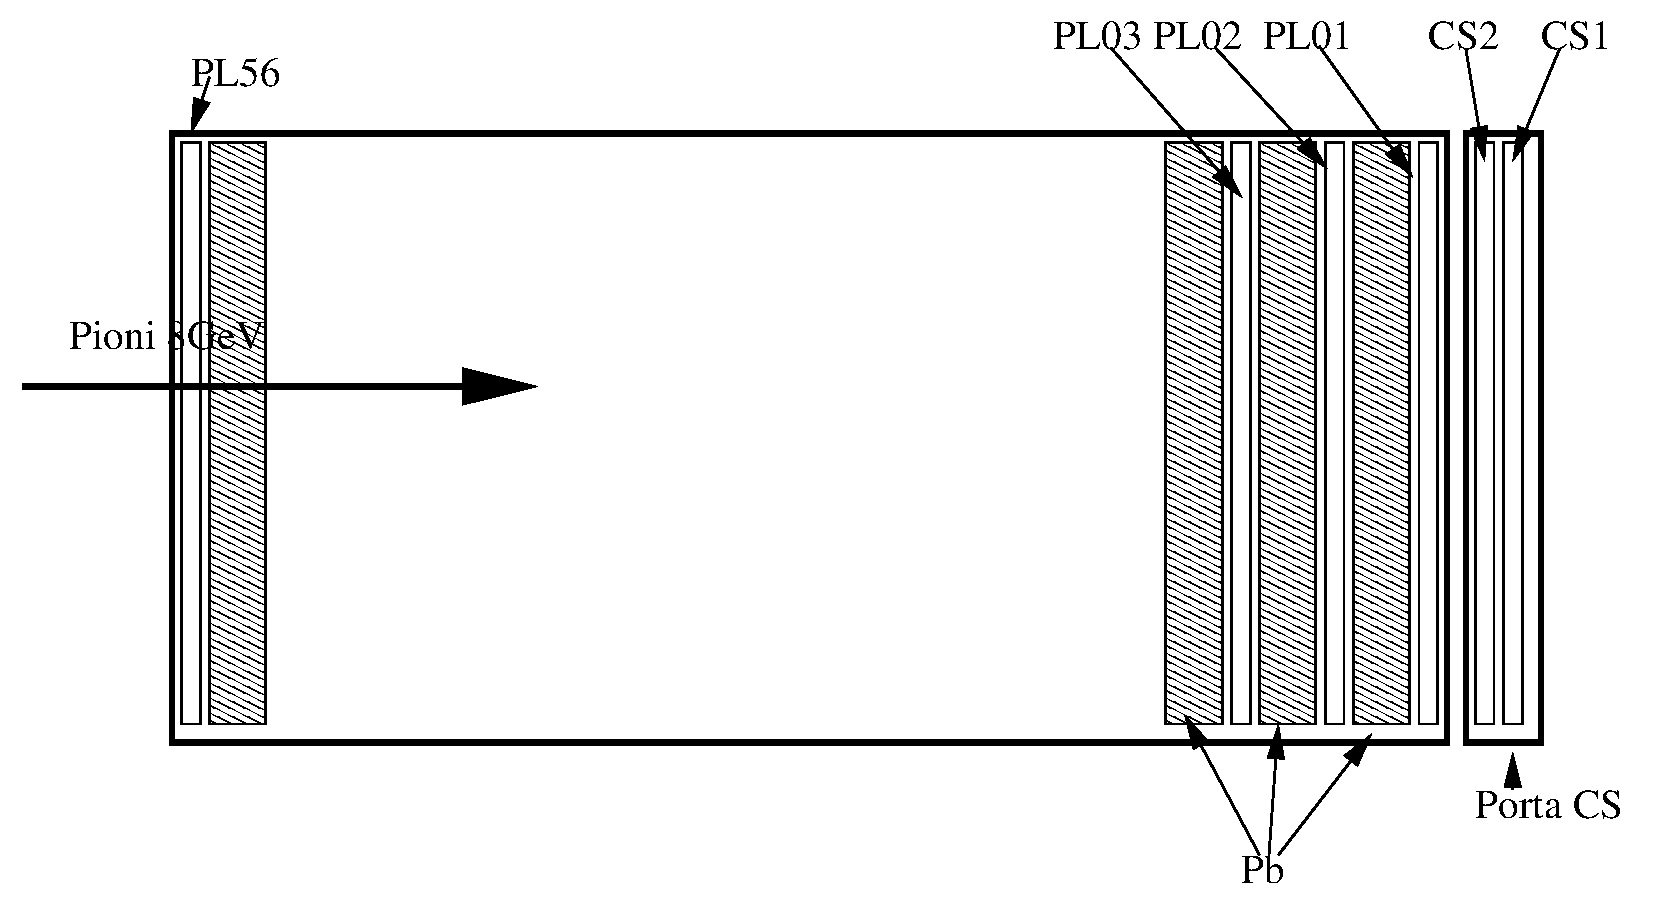
\includegraphics[width=90mm,height=90mm]{eps/brick13.eps}
\end{center}
\label{fig:brick13}
\caption{Schema brick13 }
\end{figure}



\begin{table}
\begin{center}
\begin{tabular}{||c|c|c|c||}
\hline
\hline
Brick &-150mrad& 100mrad&320mrad\\
\hline
\#13& 57398& 56734&63083\\
\hline
\end{tabular}
\label{table:brick13D}
\end{center}
\end{table}


Per le 5 lastrine del brick13 (2CS+3brick) si  � effettuato una'area di scansione di $\sim 80cm^2$ in modo da avere uno studio della connessione e planarit� su tutta la superfice e studiare eventuali effetti di bordo.

Prima della procedura di intercalibrazione occorre determinare la distanza tra le  superfici della lastrina CS2 e PL01. Questa distanza non � nota con molta precisione. Quindi si  � sviluppato un tool per la determinazione di questa distanza utilizzando le traccie a grande angolo del fascio. Si sono effettuati varie iterazioni , in modo da tener conto sia  delle rototraslazione per ogno varizione della  distanza tra i due piatti.
Il valore ottenuto da questa procedura  di� $4.7mm$. Dopo questa procedura � stato possibile effettuare la procedura di intercalibrazione dei vari piatti i, in modo da avere una misura del didiallinemanto tra le varie lastrine. In tabella \ref{table:aff} sono riportate le trasformazioni affini, riferite al CS1, dei vari piatti ottenute dalla procedura di intercalibrazione. Mentre in tabella \ref{table:aff1} sono riporrtate le trasfromazioni affini di un piatto rispetto ad un altro.

\begin{table}
\begin{center}
\begin{tabular}{||c|c|c|c|c|c|c|c||}
\hline
Piatto&Z&A11&A12&B1&A21&A22&B2\\
\hline
CS1&-7900&1.0&0.0&0.0&1.0&0.0&0.0\\
\hline
CS2 &-7600&0.999963&-0.009357&0.009699&0.9999897&-35.041355&-11.182884\\
\hline
PL01&-2600&1.000682&-0.018341&0.018584&1.0026976&78.772865&-1039.353271 \\
\hline
PL02& -1300&1.000722&-0.007328&0.008518&1.003592&-72.062424&-956.398071\\
\hline
PL03& 0&1.000836&-0.007328&0.008518&1.003592&-74.062424&-956.398071\\
\hline

\end{tabular}
\end{center}
\caption{Trasformazioni affini rispetto al CS}
\label{table:aff}
\end{table}




\begin{table}
\begin{center}
\begin{tabular}{||c|c|c|c|c|c|c|c||}
\hline
Piatto&Z&A11&A12&B1&A21&A22&B2\\
\hline
CS2 &-7600&0.999963&-0.009357&0.009699&0.9999897&-35.041355&-11.182884\\
\hline
PL01&-2600&1.000682&1.000765&-0.008784&1.002806&94.667931&-1030.047852 \\
\hline
PL02& -1300&1.000255&0.004211&-0.003501&1.000555&-55.183800&23.849262\\
\hline
PL03& 0&1.000010&0.006728&-0.006572&1.000162&-67.190315&58.578827\\
\hline
\end{tabular}
\end{center}
\caption{Trasformazioni affini rispetto al piatto precedente}
\label{table:aff1}
\end{table}

           

Dalla tabella \ref{table:aff1} si nota che il disallineamento tra i due CS �
 contenuto in poche decine di micron, dello stesso ordine di grandezza del disallineamento tra le lastre del brick. Mentre per quanto riguarda il CS2 e PL01 abbiamo un disallineamento di poco pi� $1mm$ solo nella direzione $Y$. 


\begin{figure}[!tbp]
\begin{center}
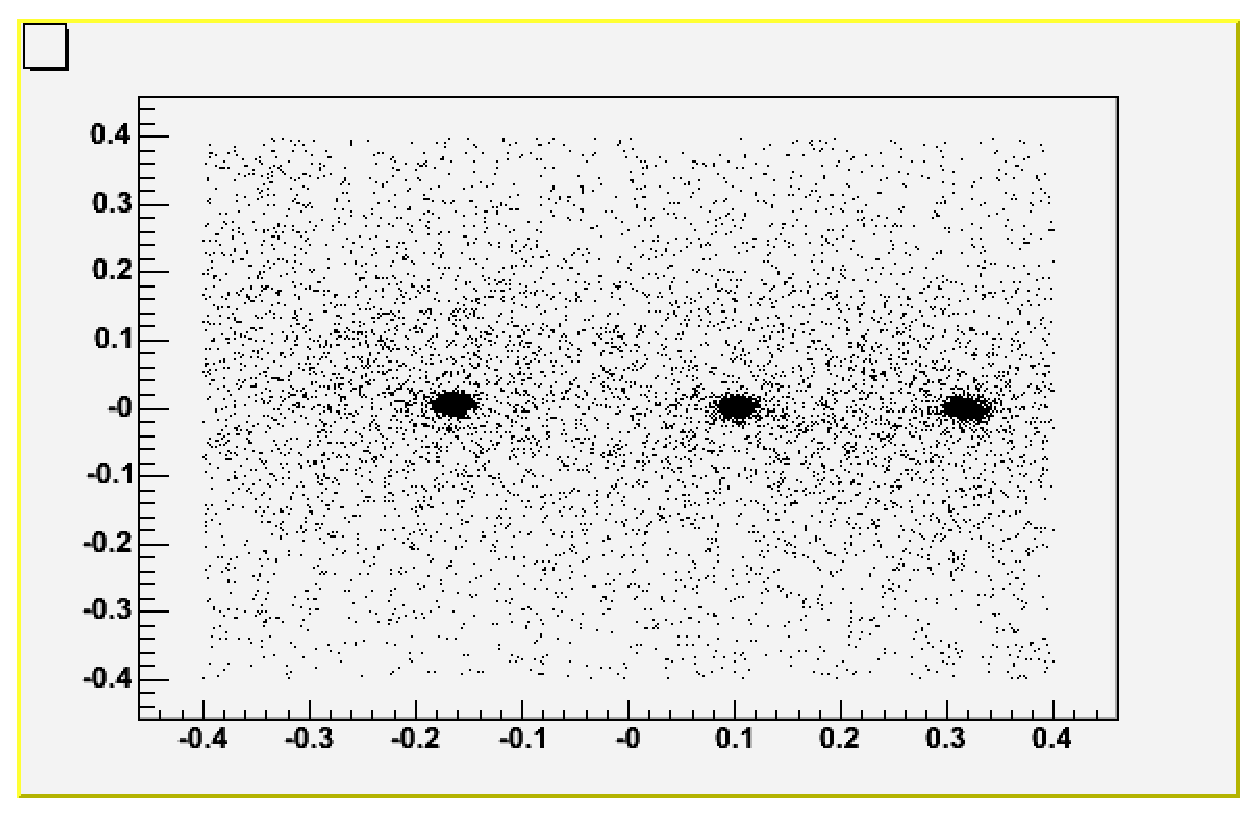
\includegraphics[width=90mm,height=90mm]{eps/peak_b13.eps}
\end{center}
\label{fig:b13txty}
\caption{Distribuzione angolare  }
\end{figure}


Si � anche studiata l'efficienza di tracciamento per i vari angoli per il piatto PL03. In tabella \ref{table:eff} sono riportati i valori ottenuti per i vari angoli. I valori ottenuti sono confrontabili  con quelli ottenuti in tabella \ref{table:eff}, oltretutto tenendo conto della gap di $4.7mm$ tra il CS2 e PL01.



\begin{table}
\begin{center}
\begin{tabular}{||c|c|c|c|c||}
\hline\hline
Angolo&tx(rad) &eff\\
\hline
P00& 0.320&$85.9 \pm0.63$\\
\hline
P01&0.100&$91.6 \pm 0.45$\\
\hline
P02&-0.160&$88.9 \pm 0.65$\\
\hline\hline
\end{tabular}
\label{table:effcs}
\caption{Misura di efficienza di ricotruzione a vari angoli. }
\end{center}
\end{table}






{\Huge Profile}



\begin{figure}[tbp]
\begin{center}
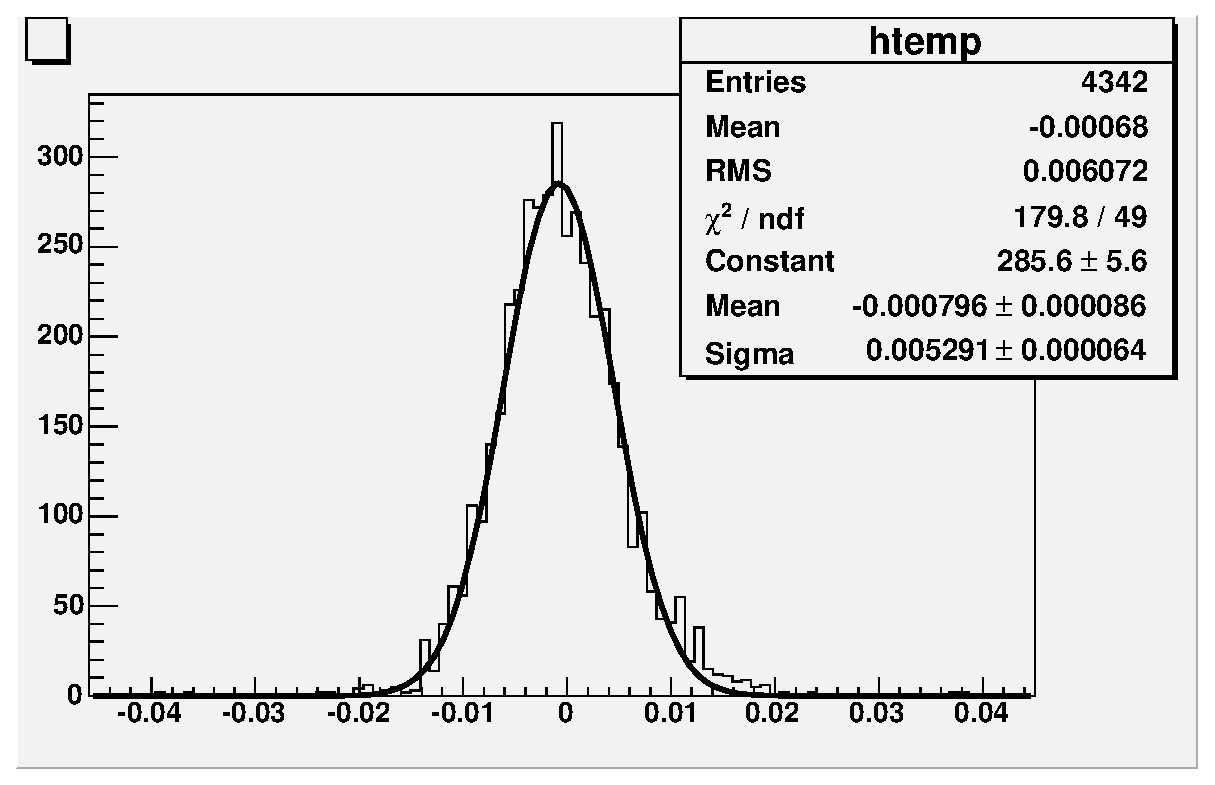
\includegraphics[width=90mm,height=90mm]{eps/CStx0.eps}
\end{center}
\caption{Differenza angolare nella proezione X $\theta=320mrad$  }
\end{figure}

\begin{figure}[tbp]
\begin{center}
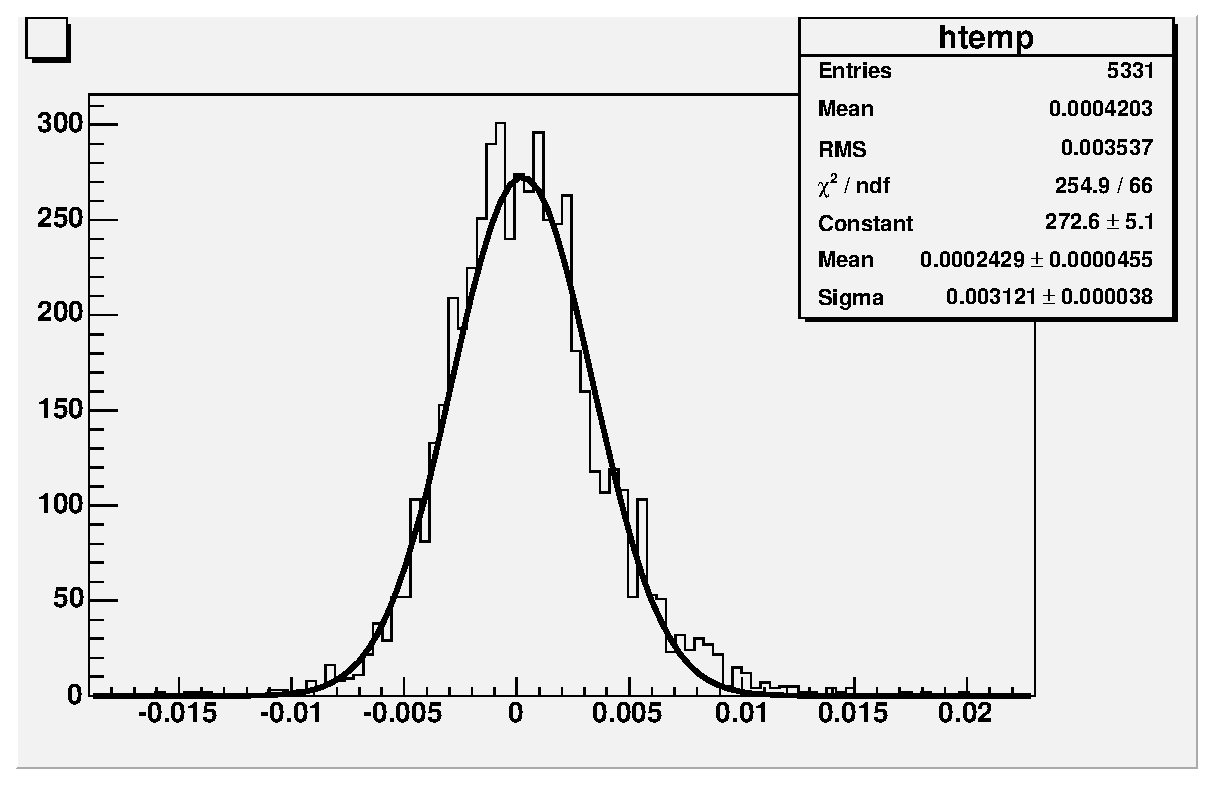
\includegraphics[width=90mm,height=90mm]{eps/CStx1.eps}
\end{center}
\caption{Differenza angolare nella proezione X $\theta=100mrad$  }
\end{figure}

\begin{figure}[tbp]
\begin{center}
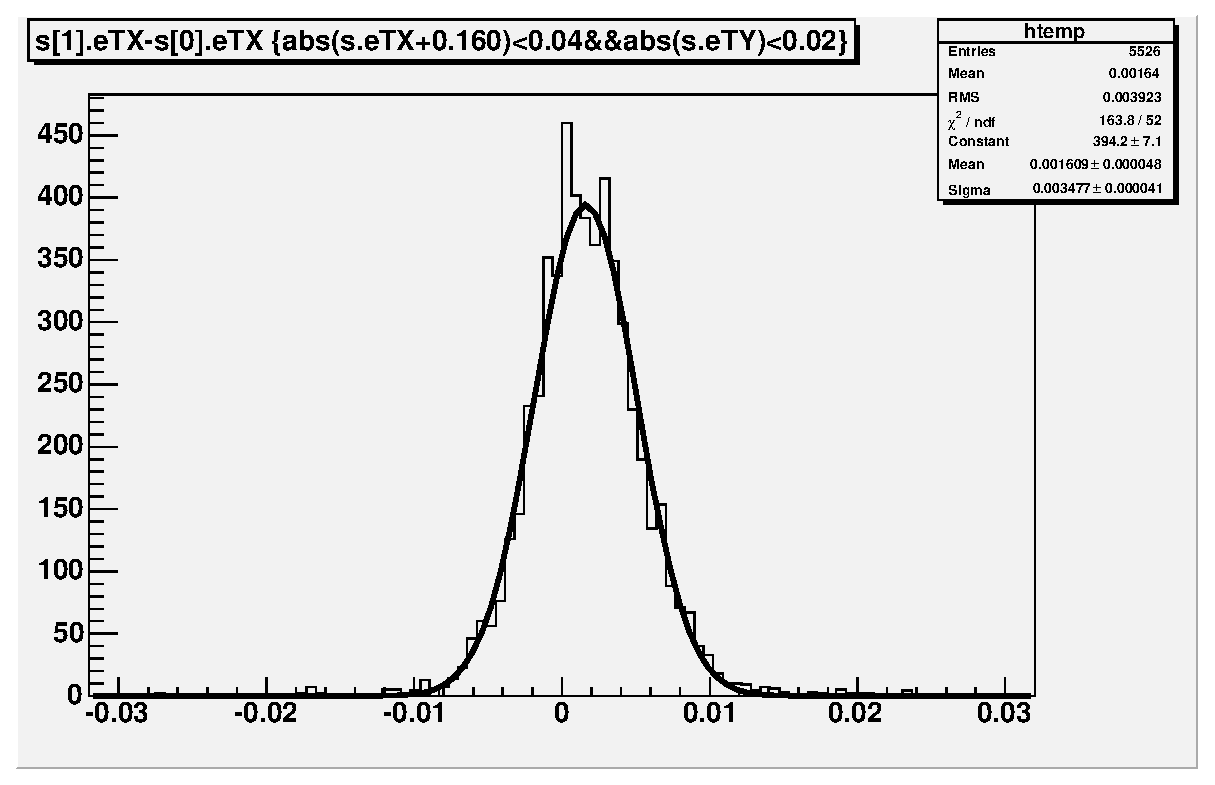
\includegraphics[width=90mm,height=90mm]{eps/CStx2.eps}
\end{center}
\caption{Differenza angolare nella proezione X $\theta=-150mrad$  }
\end{figure}

\begin{figure}[tbp]
\begin{center}
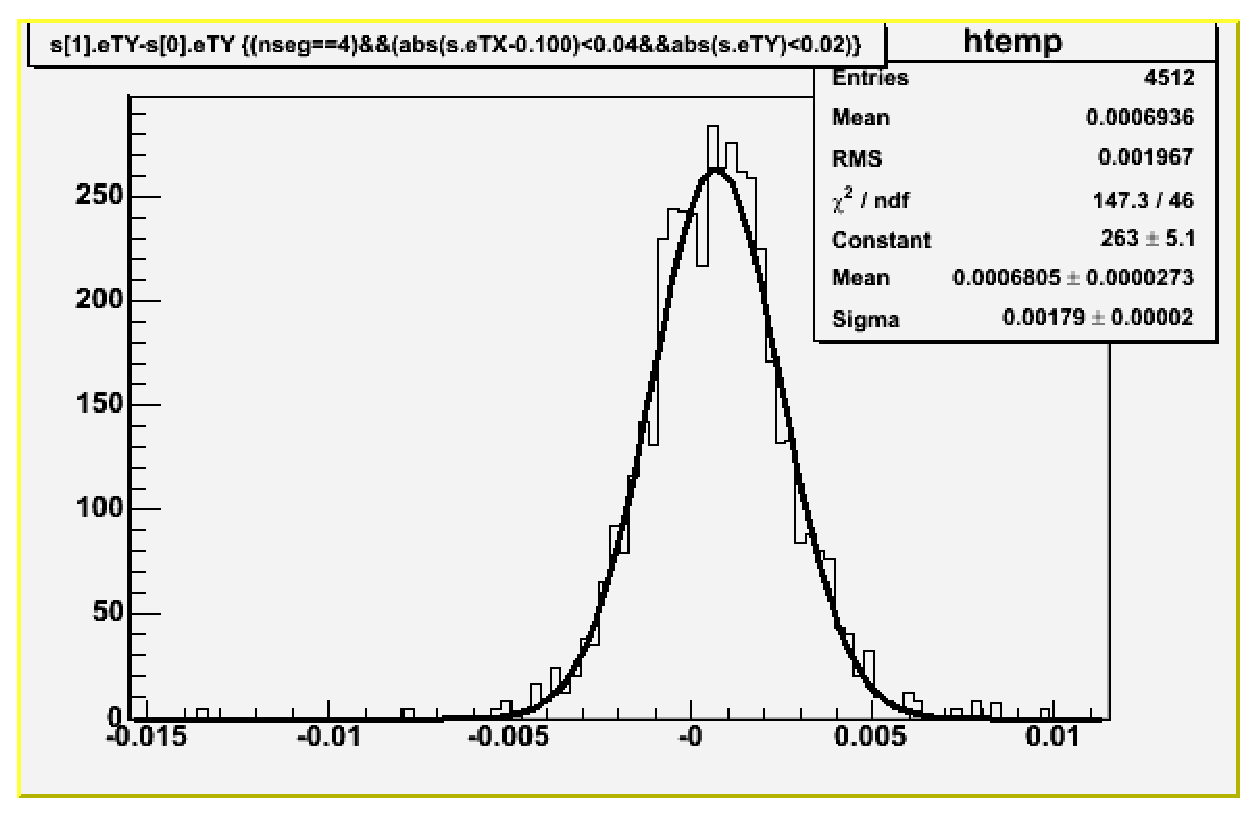
\includegraphics[width=90mm,height=90mm]{eps/CSty.eps}
\end{center}
\caption{Differenza angolare nella proezione X $\theta=-150mrad$  }
\end{figure}

\begin{figure}[tbp]
\begin{center}
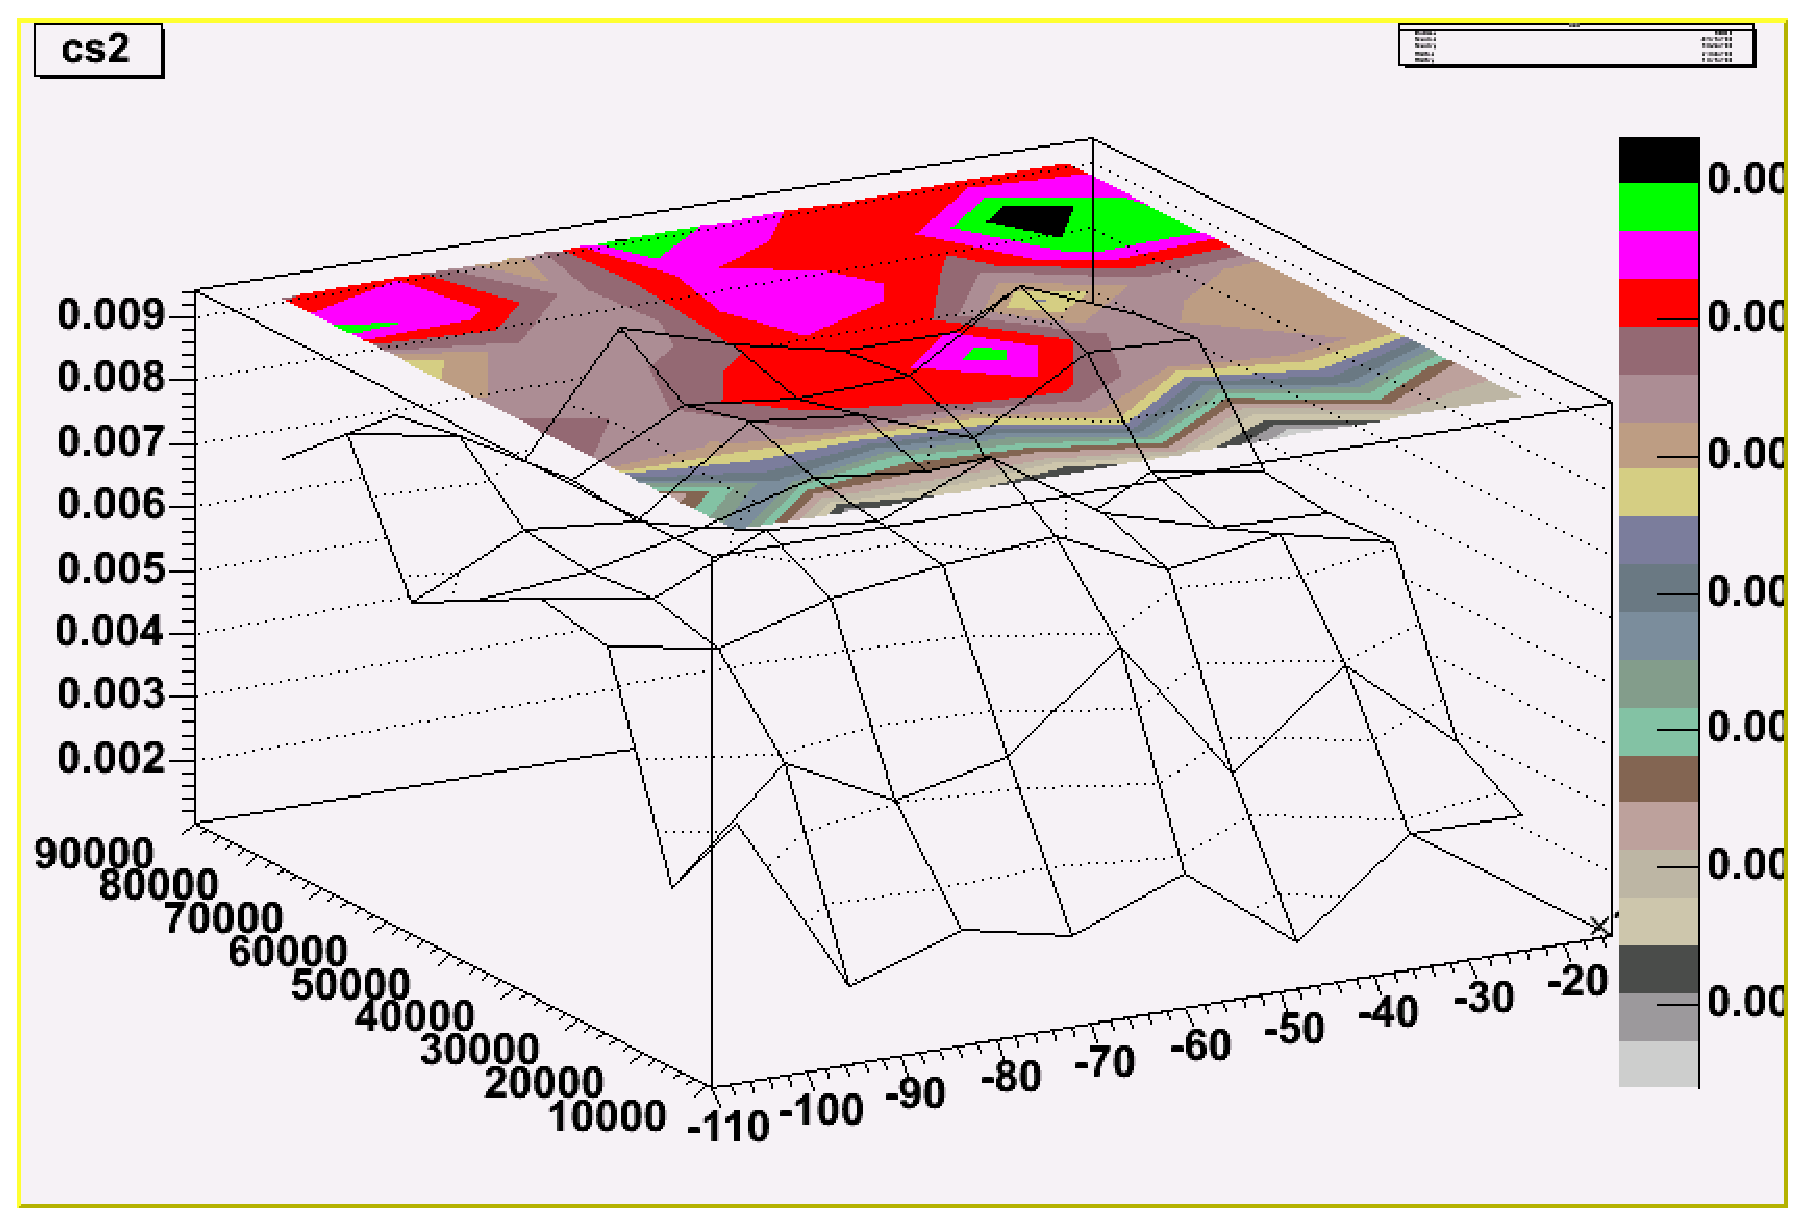
\includegraphics[width=90mm,height=90mm]{eps/cs1_2_b13.eps}
\end{center}
\caption{Planarita' dei due cs sulla tutta la superfice}
\end{figure}

\section{Connessione due CS , brick dummy}

